\documentclass[11pt,English]{article}
\usepackage[utf8]{inputenc}
\usepackage{amsmath}
\usepackage[bottom]{footmisc}
\usepackage{graphicx}


% Keywords command
\providecommand{\keywords}[1]
{
  \small	
  \-\ \-\ \-\ \textbf{\textit{Keywords --}} #1
}

% Plot set up --Thomas--
\usepackage{pgfplots}
\usetikzlibrary{external}
\tikzexternalize[prefix=tikz/]
\pgfplotsset{compat=1.16,scale=1.25}

\pgfplotsset{
    vector/.style={
        % Axis Line setup
        axis lines=center,
        axis line style={latex-latex},
        % View Set up, to rotate the graph
        view={0}{90},
    }
}





% Slides 
% 
% 1) Authors names and affiliations
% 2) Title abstract keywords
% 3) 147 why its important
%
% History
%
% http://mathshistory.st-andrews.ac.uk/Biographies/Green.html
%
%
%
% Example I
% - Apex Calc III - example "Confirming Green's Theorem" pg. 875
%     https://www.apexcalculus.com/downloads
%
%
%
%
% Example II
%
% 
% https://brilliant.org/wiki/greens-theorem/
%https://www.khanacademy.org/math/multivariable-calculus/greens-theorem-and-stokes-theorem/greens-theorem-articles/a/greens-theorem-examples
%
%

\title{
Green's Theorem\\
    \large Historical Origins and Analytical Applications\\
    \small MATH 147 Final Project\\
    \small University of Kansas, Dept. of Mathematics
}
\author{
    Atkins, Thomas\\
    \texttt{thomas.atkins@ku.edu}
    \and
    Mills, Garrett\\
    \texttt{glmdev@ku.edu}
    \and
    Weng, QiTao\\
    \texttt{wengqt@ku.edu}
}
\date{December 2019}

\begin{document}

\maketitle
\begin{abstract}
    In which the authors investigate the historical origins and several mathematical applications of the commonly known Green's theorem. Discovered by George Green in the late 1820s, this theorem provides a relationship between the line integral of a particular curve and the surface integral of its enclosed region. Green's theorem is closely related to the divergence theorem, and is simply a specific case of the more general Stoke's theorem. Beyond basic applications to flux and surface integrals, Green's theorem can be reverse applied to calculate difficult-to-evaluate area calculations. It also plays an integral role (pun intended) in the proof of other important theorems.
\end{abstract}

\keywords{Green, Stoke, integration, vector calculus}

\section{Introduction}

George Green, the mathematician who would go on to postulate the now famous Green's theorem, was born in July of 1793. As a youth he received only a year of formal schooling when he was 8 years old. While working full time at a mill owned by his father in 1728 he published \emph{An Essay on the Application of Mathematical Analysis to the Theories of Electricity and Magnetism.} In that publication, Green would put forth the theorem that now bears his name, though it would be years before anyone would fully appreciate it. The publication of the paper would catch the eye of one Sir Edward Bromhead, who would later encourage Green to study Mathematics at Cambridge. He would died before his work would be recognized as the landmark discovery it was.\footnote{"George Green
" University of St Andrews, October 1998, (http://mathshistory.st-andrews.ac.uk/Biographies/Green.html)}

\begin{figure}
    \centering
    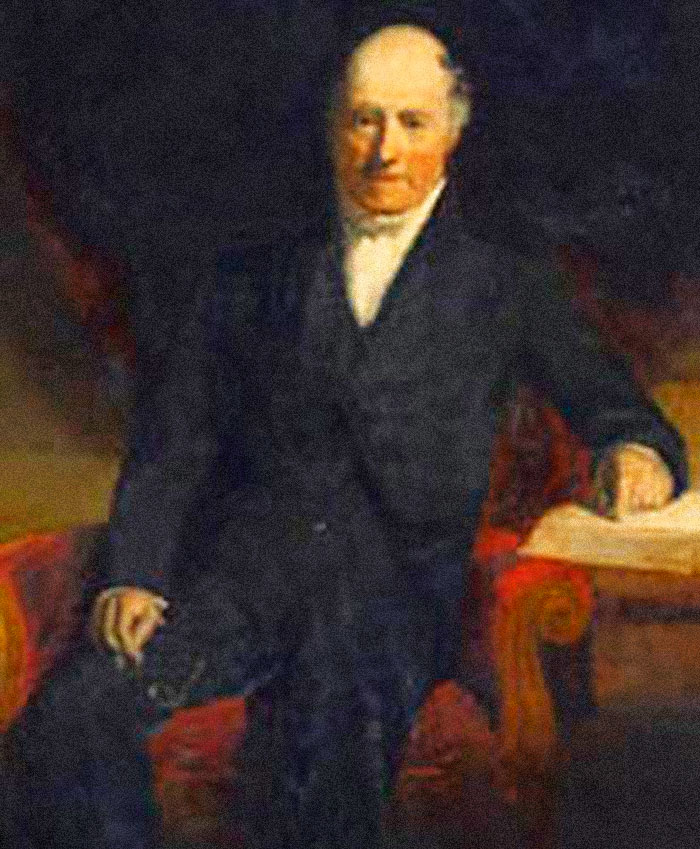
\includegraphics[scale=.2]{George_Green.jpg}
    \caption{George Green (http://georgegreens.com/history-george-greens.html)}
    \label{fig:my_label}
\end{figure}


\subsection{Definition}
% here is some definitions stuffs
Green's theorem is commonly defined as follows.\footnote{"Section 5-7: Green's Theorem" - Paul Dawkins, Lamar University - 02-22-2019. (http://tutorial.math.lamar.edu/Classes/CalcIII/GreensTheorem.aspx)} Let $C$ be a simple, smooth, closed, positively-oriented curve and $D$ the region enclosed by said curve. Assume $P$ and $Q$ are, at least, singly differentiable. Then, the following relationship holds:
$$
\int_C{ P dx + Q dy } = \iint_D{ \left( \frac{\partial Q}{\partial x} - \frac{\partial P}{\partial y} \right) dA }
$$
Essentially, this theorem defines a relationship between the quantity of a vector field that "passes through" a boundary and the differential of that vector field across the surface enclosed by that boundary. This is useful because, often, a difficult-to-calculate line integral can be made much simpler by converting them to a double-integral using Green's theorem (and vice-versa).

\subsection{Connections to Stoke's Theorem}
Interestingly, Stoke's theorem and Green's theorem are closely related. While it is technically accurate to say that Green's theorem is a specific, 2-dimensional application of Stoke's theorem, in actuality, Stoke's theorem is a 3-dimensional generalization of the earlier Green's theorem.\footnote{"The Idea Behind Stoke's Theorem" - Dr. Duane Nykamp et al., Math Insight - n.d. (https://mathinsight.org/stokes\_theorem\_idea)}

While, if you have a surface in the xy-plane, Green's theorem can be used to calculate the circulation of some field through the boundary of that surface, Stoke's generalization of Green's theorem can be used if your surface exists in the z-dimension as well. In this case, the curl of the vector field (which is used by Stoke's theorem) is analogous to the cross-variable partial differentials used by Green's implementation.

\subsection{Connections to Divergence Theorem}
\begin{align*}
    \oint_C \vec{F} \cdot \vec{n} \; ds = \iint_D div \; \vec{F} \; dA
\end{align*}
Above is the generally accepted definition of the divergence theorem.\footnote{"Flow, Flux, Green’s Theorem and the Divergence Theorem" - Dr. Timothy Prescott, Apex Calculus - n.d. (https://sites.und.edu/timothy.prescott/apex/web/apex.Ch15.S4.html)} It relates the circulation of some vector field across the surface to the integral sum of all the closed loops over that surface. As with Stoke's theorem, the divergence theorem is simple a more generalized statement of the same kernel idea as Green's theorem. Assume, for example, the following 2-dimensional vector field:
$$
\vec{f} = \left<P,Q\right>
$$

If we dot this field with its normal, we're left with an expression that might look familiar:
$$
\vec{F} \cdot \hat{n} = P \; dy - Q \; dx
$$

This is because the statement of Green's theorem can be derived from the divergence theorem by isolating the divergence theorem to 2 dimensions and evaluating it with general variables. It is evident that Green's theorem was an important milestone in the development of vector analysis which enabled the generalization of higher-dimension theorems like the divergence theorem and Stoke's theorem.

\section{Verification of Green's Theorem}
Green's theorem is commonly used in applications of vector calculus to other fields of study, particularly physics in the plane. One example of this is calculating the circulation of vector fields along a closed boundary. For our purposes, circulation refers to the magnitude of the vector field that \emph{passes through} or \emph{pushes against} the closed boundary.\footnote{"Vector Calculus: Understanding Circulation and Curl" - Editors of BetterExplained, BetterExplained, Vector Calculus - n.d. (https://betterexplained.com/articles/vector-calculus-understanding-circulation-and-curl/)}



% ==== Illustration Image of Circulation Here ====

\begin{figure}[h]
    \centering
        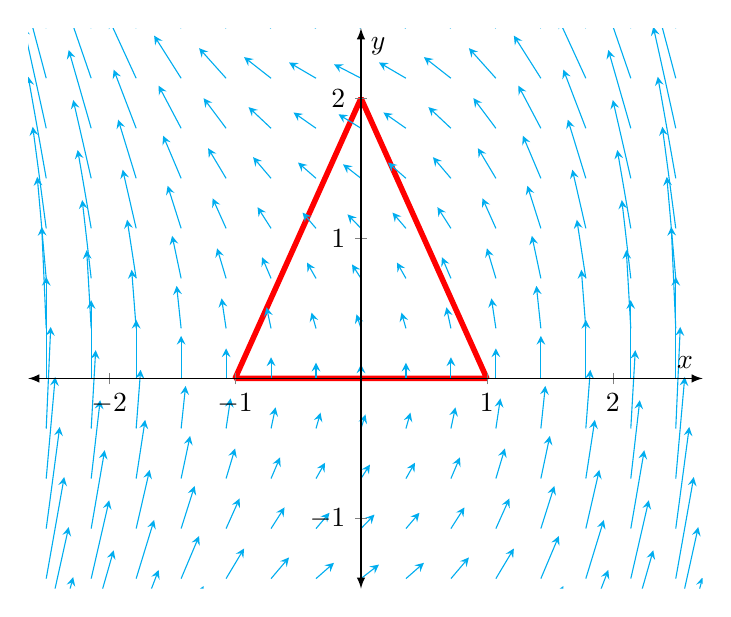
\begin{tikzpicture}
            \begin{axis}[vector,
                title={},
                domain=-2.5:2.5,
                ymin = -1.5,
                ymax = 2.5,
                xlabel=$x$,
                ylabel=$y$,
            ]
                \addplot[
                    patch,
                    patch type=triangle,
                    color = white,
                    line width=2pt,
                    faceted color=red,
                ] 
                    coordinates {
                        (-1,0)
                        (1,0)
                        (0,2)
                    };
                \addplot3[
                    cyan,
                    quiver={
                        u={-y},
                        v={x^2+1},
                        scale arrows=0.1
                    },
                    -stealth,
                    samples=15]
                    {x};
            \end{axis}
        \end{tikzpicture}
    \caption{Illustration of Circulation}
    \label{Circulation}
\end{figure}



Take, for example, the field and boundary pictured above. There is some vector field in the plane, $\vec{E}$, that emanates from some point $P$. Inset in that field is some simple, closed boundary $\partial S$. The circulation of the field $\vec{E}$ with respect to the boundary $\partial S$ is the magnitude $E$ that is incident on $\partial S$. That is, the \emph{amount} of the field that passes through the boundary.

We can verify Green's theorem by calculating the circulation of a vector field manually using line integrals, and using the formula for Green's. Let, for example, our electric field $\vec{E} = \left< -y, x^2+1 \right>$. The boundary, as shown above, is a triangle traversed counter-clockwise, with vertices at $\left( -1, 0 \right)$, $\left( 1, 0 \right)$, and $\left(0, 2\right)$.

\subsection{Using Line Integrals}
We can calculate the circulation using a series of line integrals of parameterizations along the sides of the triangle. Provided that you traverse it counter-clockwise, you can start at any of the vertices. Starting at $\left(-1, 0\right)$, we can use the following parameterizations:
\begin{align}
\vec{r}_1(t) &= \left<2t-1, 0\right> \;\;\;\;\; 0 \leq t \leq 1 \\
\vec{r}_2(t) &= \left<1-t, 2t\right> \;\;\;\;\;\; 0 \leq t \leq 1 \\
\vec{r}_3(t) &= \left<-t, 2-2t\right> \;\;\;\; 0 \leq t \leq 1
\end{align}

The circulation along a single edge (one of the $\vec{r}_i$) can be computed using the following vector line integral:
$$
\Phi_i = \int_{C_i} \vec{E}(\vec{r}_i) \cdot d\vec{r}_i
$$

In each case, the $d\vec{r}_i$ can be computed as $\frac{\partial\vec{r}_i}{\partial t}$. Hence, for our purposes, the various $d\vec{r}_i$ are as follows:
\begin{align}
    \frac{\partial\vec{r}_1}{\partial t} &= \left<2, 0\right> \\
    \frac{\partial\vec{r}_2}{\partial t} &= \left<-1, 2\right> \\
    \frac{\partial\vec{r}_3}{\partial t} &= \left<-1, -2\right>
\end{align}

So we can calculate the various $\Phi_i$ using the formula above. Then, we can find the resultant $\Phi_{net}$ as the sum of the circulations of the individual components.\footnote{This makes an intuitive sense. If you have a bucket with 2 liters of water per second flowing in the top and 1 liter of water per second flowing out the bottom, the total flow of water in the bucket is a gain of 1 liter of water per second ($2 \frac{L}{s} - 1 \frac{L}{s} = 1 \frac{L}{s}$).}

\begin{align*}
    \Phi_1 &= \int_{C_1} \vec{E}(\vec{r}_1) \cdot d\vec{r}_1 \\
    &= \int_0^1 \left<0, (2t-1)^2 +1\right> \cdot \left<2,0\right> dt \\
    &= 0
\end{align*}

\begin{align*}
    \Phi_2 &= \int_{C_2} \vec{E}(\vec{r}_2) \cdot d\vec{r}_2 \\
    &= \int_0^1 \left<-2t, (1-t)^2 +1\right> \cdot \left<-1,2\right> dt \\
    &= \int_0^1 (2t + 2(1-t)^2 +2) \; dt \\
    &= \int_0^1 (2t^2 -2t + 4) \; dt \\
    &= \frac{2}{3}t - t^2 + 4t \vert_0^1 \\
    &= \frac{11}{3}
\end{align*}

\begin{align*}
    \Phi_3 &= \int_{C_3} \vec{E}(\vec{r}_3) \cdot d\vec{r}_3 \\
    &= \int_0^1 \left<2t-2, t^2 +1\right> \cdot \left<-1, -2\right> \\
    &= \int_0^1 -2t-2t^2 \; dt \\
    &= -t^2 -\frac{2}{3}t^3 \mid_0^1 \\
    &= -\frac{5}{3}
\end{align*}

We can then compute the total $\Phi_{net}$ as the sum of the fluxes across the three boundary-components. That is, $\Phi_net = \Phi_1 + \Phi_2 + \Phi_3 = 0 + \frac{11}{3} - \frac{5}{3} = 2$. This result indicates that the flux of the electric field has a magnitude of 2 across the described boundary. Typically, the units for electric flux are Volt-meters ($Vm$).

\subsection{Using Green's Theorem}
As mentioned above, Green's theorem relates the circulation of a vector field over a boundary to the area of the curl of that field over the surface enclosed by the boundary. We can verify the result gained above, then, by calculating the following double-integral:
\begin{align*}
    \int_C \vec{E}(\vec{r}) \cdot d\vec{r} = \iint_D \nabla \times \vec{E} \cdot dA
\end{align*}

We begin by computing the curl of $\vec{E}$ as the virtual cross-product of the nabla-operator against the components of $\vec{E}$:
\begin{align*}
    \nabla \times \vec{E} &=
    \begin{vmatrix}
        \hat{i} & \hat{j} & \hat{k} \\
        \frac{\partial}{\partial x} & \frac{\partial}{\partial y} & \frac{\partial}{\partial z} \\
        -y & x^2 + 1 & 0
    \end{vmatrix} \\
    &= \left<0,0,2x+1\right>
\end{align*}

Now, we can compute the related area by dotting this result with the differential area. Because the boundary lies in the xy-plane, we can take the z-component for our integrand. Thus, the circulation across the boundary can be calculated as such:
\begin{align*}
    \Phi_{net} &= \iint_D \nabla \times \vec{E} \cdot dA \\
    &= \int_0^2 \int_{y/2-1}^{1-y/2} 2x+1 \; dx \; dy \\
    &= \int_0^2 2-y \; dy \\
    &= 2
\end{align*}

Thus, the circulation across the boundary is $2 \; Vm$, which is consistent with the result we found above.

\section{Applications}
Calculating parametric curves using Green's theorem instead of directly computing a line integral can often be much simpler. Calculating the area of a seashell-like spiral:\footnote{Editors of khanacademy.org. (n.d.). Green's theorem examples. Retrieved from https://www.khanacademy.org/math/multivariable-calculus/greens-theorem-and-stokes-theorem/greens-theorem-articles/a/greens-theorem-examples.}
\begin{align*}
    x(t) = t\cos{t} \\
    y(t) = t\sin{t}  \\
    0<t<2\pi \\
\end{align*}

Using a pair of functions that satisfies $\frac{\partial Q}{\partial x} - \frac{\partial P}{\partial y} = 1$, such as: $\oint_{c}-\frac{1}{2}y \; dx+\frac{1}{2}x \; dy $
\begin{align*}
    xdy-ydx &= (x(t)\frac{dy}{dt}-y(t)\frac{dx}{dt})dt \\
    &= (t\cos{t}\frac{d(t\sin{t})}{dt}-t\sin{t}\frac{d(t\cos{t})}{dt}\;dt \\
    &= (t\cos{t}(t\cos{t}+\sin{t})-t\sin{t}(-t\sin{t}+\cos{t}))\;dt \\
    &= (t^2\cos^2{t}+t\cos{t}\sin{t}+t^2\sin^2{t}-t\sin{t}\cos{t})\;dt\\
    &= (t^2(\sin^2{t}+\cos^2{t})\;dt \\
    &= t^2\:dt \\
    \int_{spiral}\frac{1}{2}(xdy-ydx) &= \int^{2\pi}_{0}\frac{1}{2}t^2dt = \frac{1}{6}t^3\Big|^{2\pi}_{0} \\
    &= \frac{4\pi^3}{3}
\end{align*}
Otherwise, in order to solve the area enclosed by the spiral, we would need to evaluate:
\begin{align*}
    \text{Area} &= \int^{2\pi}_{0} t\cos{t}\cdot (t\sin{t})'\:dt \\
    &= \int^{2\pi}_{0}t\cos{t}\cdot (t\cos{t}+\sin{t})\:dt \\
    &= \int^{2\pi}_{0} t^{2}\cos^{2}{t}+t\sin{t}\cos{t}\:dt
\end{align*}
Which results in a far more complex series of steps to the solution.

A second example can be shown with a squashed ellipse, or what appears to be an hourglass, with the parameterization:\footnote{Editors of brilliant.org. (n.d.). Green's Theorem. Retrieved from https://brilliant.org/wiki/greens-theorem/.}
\begin{align*}
    x &= \sin{\theta} \\
    y &= \sin^2{\theta}\cos{\theta} \\
    0 &< \theta < 2\pi \\
    \oint_{c}y\:dx &= \int^{2\pi}_{0}(\sin^2{\theta}\cos{\theta})(\cos{\theta})\:d\theta \\
\end{align*}


\end{document}
